%; whizzy paragraph -pdf xpdf -latex ./whizzypdfptex.sh
%; whizzy-paragraph "^\\\\begin{frame}\\|\\\\emtext"
% latex beamer presentation.
% platex, latex-beamer $B$G%3%s%Q%$%k$9$k$3$H$rA[Dj!#(B 

%     Tokyo Debian Meeting resources
%     Copyright (C) 2012 Junichi Uekawa

%     This program is free software; you can redistribute it and/or modify
%     it under the terms of the GNU General Public License as published by
%     the Free Software Foundation; either version 2 of the License, or
%     (at your option) any later version.

%     This program is distributed in the hope that it will be useful,
%     but WITHOUT ANY WARRANTY; without even the implied warreanty of
%     MERCHANTABILITY or FITNESS FOR A PARTICULAR PURPOSE.  See the
%     GNU General Public License for more details.

%     You should have received a copy of the GNU General Public License
%     along with this program; if not, write to the Free Software
%     Foundation, Inc., 51 Franklin St, Fifth Floor, Boston, MA  02110-1301 USA

\documentclass[cjk,dvipdfmx,12pt]{beamer}
\usetheme{Tokyo}
\usepackage{monthlypresentation}

%  preview (shell-command (concat "evince " (replace-regexp-in-string "tex$" "pdf"(buffer-file-name)) "&")) 
%  presentation (shell-command (concat "xpdf -fullscreen " (replace-regexp-in-string "tex$" "pdf"(buffer-file-name)) "&"))
%  presentation (shell-command (concat "evince " (replace-regexp-in-string "tex$" "pdf"(buffer-file-name)) "&"))

%http://www.naney.org/diki/dk/hyperref.html
%$BF|K\8l(BEUC$B7O4D6-$N;~(B
\AtBeginDvi{\special{pdf:tounicode EUC-UCS2}}
%$B%7%U%H(BJIS$B7O4D6-$N;~(B
%\AtBeginDvi{\special{pdf:tounicode 90ms-RKSJ-UCS2}}

\newenvironment{commandlinesmall}%
{\VerbatimEnvironment
  \begin{Sbox}\begin{minipage}{1.0\hsize}\begin{fontsize}{8}{8} \begin{BVerbatim}}%
{\end{BVerbatim}\end{fontsize}\end{minipage}\end{Sbox}
  \setlength{\fboxsep}{8pt}
% start on a new paragraph

\vspace{6pt}% skip before
\fcolorbox{dancerdarkblue}{dancerlightblue}{\TheSbox}

\vspace{6pt}% skip after
}
%end of commandlinesmall

\title{Debian $B$H(B systemd}
\subtitle{$BEl5~%(%j%"(BDebian$BJY6/2q(B/OSC 2015 Tokyo Fall\\$BBh(B132$B2s(B 2015$BG/(B10$B7nEY(B 2$B2sL\(B}
\author{$B4d>>(B $B?.MN(B}
\date{2015$BG/(B10$B7n(B24$BF|(B}
\logo{
\includegraphics[width=8cm]{image200607/openlogo-light.eps}}

\begin{document}

\begin{frame}
\titlepage{}
\end{frame}

\begin{frame}{$B<+8J>R2p(B}
\begin{itemize}
  \item $B%=%U%H%&%'%"%(%s%8%K%"(B
  \item Debian Project Official Developer
  \item Bluez, Mozc, Erlang $B<~$j$N%Q%C%1!<%8%a%s%F%J(B
  \item 2015$BG/EY(B Debian JP Project Leader
  \item Linux kernel $B3+H/!"(BU-Boot Custodian$B!"(BXFCE $BF|K\8l%3!<%G%#%M!<%?!"(BYocto Project $B3+H/(B
 \end{itemize}
\end{frame}

\begin{frame}{Agenda}
  \begin{itemize}
   \item systemd $B$H$O(B
   \item systemd $B$X$N0\9T$H5/$-$?;vJA(B
   \item systemd $B$r;HMQ$;$:$K(B Debian $B$rMxMQ$9$k$K$O(B
   \item $B:#8e$N%$%Y%s%H(B
  \end{itemize}
\end{frame}

\section{systemd $B$H$O(B}
\emtext{systemd $B$H$O(B}

\begin{frame}{systemd}
\begin{itemize}
\item init $B%W%m%0%i%`$N0l$D(B

      init $B$H$O(B $B%+!<%M%k$,8F$V:G=i$N%W%m%0%i%`$NAm>N(B

      \end{itemize}
\end{frame}

\begin{frame}{systemd}

\begin{minipage}{0.55\hsize}
$B%V!<%H%7!<%1%s%9(B
\begin{enumerate}
\item $BEE8;EjF~(B $\rightarrow$ BIOS $B$^$?$O(B UEFI $B$,5/F0(B
\item BIOS $B$^$?$O(B UEFI $\rightarrow$  $B%V!<%H%m!<%@$r5/F0(B
\item $B%V!<%H%m!<%@(B $\rightarrow$ $B%+!<%M%k(B $B$r5/F0(B
\item $B%+!<%M%k(B $\rightarrow$ init $B$r5/F0(B
\end{enumerate}
\end{minipage}
\begin{minipage}{0.39\hsize}
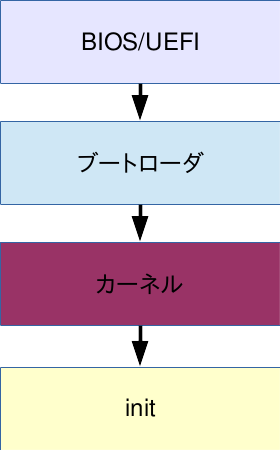
\includegraphics[width=0.8\hsize]{image201510/boot_seq.png}
\end{minipage}

\end{frame}

\begin{frame}{systemd}
\begin{itemize}
\item init $B%W%m%0%i%`$N0l$D(B

      init $B$H$O(B $B%+!<%M%k$,8F$V:G=i$N%W%m%0%i%`$NAm>N(B

\item cgroup $B$K$h$k%W%m%;%94IM}(B
\item $B%G!<%b%s$NJBNs=hM}(B
\item shell $B$r;H$o$J$$@_Dj(B
\item linux $B@lMQ(B init $B%W%m%0%i%`(B
\item Debian$B!"(BUbuntu$B!"(BRedHat $B$J$I$N<gMW(B Linux $B%G%#%9%H%j%S%e!<%7%g%s$N%G%U%)%k%H(Binit $B%W%m%0%i%`$H$7$F:NMQ$5$l$F$$$k!#(B
\end{itemize}
\end{frame}

\section{systemd $B$X$N0\9T$H(BDebian $B3&7($G5/$-$?;vJA(B}
\emtext{systemd $B$X$N0\9T$H(BDebian $B3&7($G5/$-$?;vJA(B}

\begin{frame}{2014$BG/(B2$B7n(B11$BF|(B}

\begin{itemize}
\item Debian 8.0 $B$+$i%G%U%)%k%H(B init $B%7%9%F%`(B $B$,(B sysvinit $B$+$i(B systemd $B$K!#(B
\item Debian $B5;=Q0Q0w2q!J(BDebian Technical Committee: Debian $B%W%m%8%'%/%HFb$N5;=QE*$JO@Ah$K$D$$$F:G=*H=CG$r2<$90Q0w2q!K$,7hDj$7$?$b$N!#(B

\url{https://lists.debian.org/debian-ctte/2014/02/msg00402.html}

\url{https://bugs.debian.org/727708}

\end{itemize}

\end{frame}



\begin{frame}{2014$BG/(B9$B7n(B19$BF|(B}

\begin{itemize}
\item $B%G%U%)%k%H$N(B init $B%7%9%F%`(B $B$,(B systemd $B$K$J$j!"%$%s%9%H!<%i$N%G%U%)%k%H(B $B%G%9%/%H%C%W4D6-$K4X$7$F$b:F9M$5$l$k!#(B
\item $B$=$N7k2L!"(BXfce $B$+$i(B GNOME3 $B$KJQ99$5$l$k!#(B
      \url{https://anonscm.debian.org/cgit/tasksel/tasksel.git/commit/?id=dce99f5f8d84e4c885e6beb4cc1bb5bb1d9ee6d7}
      \footnote{init $B%7%9%F%`(B $B$,(B systemd $B$G$J$/$F$b(B GNOME3$B$OF0:n$9$k!#(B}

\end{itemize}

\end{frame}

\begin{frame}{2014$BG/(B10$B7n(B16$BF|(B}

\begin{itemize}
\item Ian Jackson $B$,(B init $B%7%9%F%`$NA*Br$N<+M3$r;D$7$F$*$/$Y$-$G$O!"$H(B
systemd$B$r;HMQ$7$J$$%7%9%F%`$N%5%]!<%H$r%Q%C%1!<%8%a%s%F%J$K5a$a$k0lHL7h5D$rDs0F!#(B
\item $B;Y;}<T$,=8$^$j!"0lHL7h5D$,9T$o$l$k$3$H$K$J$C$?$,!"7k2LIT@.N)!#(B

\url{https://lists.debian.org/debian-vote/2014/10/msg00001.html}

\item Jessie $B%U%j!<%:D>A0$G$NDs0F$KITK~$,=P$k!#(B
\item $B5;=Q7hDj%W%m%;%9$NLdBj$,O*Dh$5$l$k!#(B

\end{itemize}

\end{frame}

\begin{frame}{$B$=$N7k2L!D(B}


\begin{itemize}
\item Joey Hess $B$,(B Debian Developer $B$r<-$a$k(B

debconf$B!"(Bdebhelper$B!"(Balian$B!"(Bikiwiki $B$J$I$N3+H/<T(B

\item Colin Watson$B!"(BRuss Allbery$B!"(BIan Jackson $B$,(B Debian $B5;=Q0Q0w2q(B $B$r<-$a$k(B
\item Tollef Fog Heen $B$,(B systemd $B%a%s%F%J$+$i<-$a$k(B

$B$=$N8e(B Debian $B5;=Q0Q0w2q(B $B%a%s%P$K!#(B

\end{itemize}

\end{frame}

\begin{frame}{2014$BG/(B11$B7n(B28$BF|(B}

$B$=$7$F(B Devuan$B%W%m%8%'%/%H$,N)$A>e$,$k!#(B

\begin{center}

\includegraphics[width=1\hsize]{image201510/Devuan-logo.png}
\end{center}

\begin{itemize}
\item Debian $B%Y!<%9$N(B systemd $B$r;H$o$J$$(BOS$B$rDs6!$9$k%W%m%8%'%/%H(B
\item i386, amd64, armhf $B$N%$%a!<%8$H%$%s%9%H!<%i$rHRI[(B
\item udev $B$NBeBX%W%m%0%i%`$G$"$k(Bvdev$B$r3+H/(B
\item \url{http://files.devuan.org/}
\end{itemize}

\end{frame}

\begin{frame}[containsverbatim]

\begin{itemize}

\item 2015/4/21 Ubuntu 15.04 $B%j%j!<%9(B

    init $B%7%9%F%`$K(B systemd $B$r:NMQ$7$?$O$8$a$F$N%j%j!<%9(B

\item 2015/4/25 Debian 8.0 ($B%3!<%I%M!<%`(B Jessie$B!K%j%j!<%9(B

\end{itemize}

\end{frame}

\begin{frame}
\begin{itemize}
\item $BM%=($J3+H/<T$,%W%m%8%'%/%H$J$I$+$iH4$1$k(B
\item Devuan $B%W%m%8%'%/%H$,N)$A>e$,$k(B
\item $B$=$l$G$b(B Debian 8.0 $B$OM=DjDL$j%j%j!<%9$5$l$?(B
\end{itemize}
\end{frame}

\section{systemd $B$r;HMQ$;$:$K(B Debian $B$rMxMQ$9$k$K$O(B}
\emtext{systemd $B$r;HMQ$;$:$K(B Debian $B$rMxMQ$9$k$K$O(B}

\begin{frame}[containsverbatim]
Debian $B$G$O(B systemd $B$K$J$C$F$b%G!<%b%s$KBP$9$kA`:nJ}K!$OJQ$o$i$J$$(B

\begin{itemize}
\item $BNc(B: apache2 start
\begin{commandline}
$ sudo service apache2 start
\end{commandline}

\item $BNc(B: apache2 stop
\begin{commandline}
$ sudo service apache2 stop
\end{commandline}

\end{itemize}

\end{frame}

\begin{frame}[containsverbatim]{sysvinit $B$X$N@Z$jBX$((B}

Debian $B$N(B init $B%7%9%F%`$r(B sysvinit $B$K@Z$jBX$($?$$!#(B

\begin{itemize}
\item systemd $B7y$$(B
\item sysvinit $B$N$[$&$K47$l$F$$$k(B
\item $BFH<+%5!<%S%9%a%s%F%J%s%9$N$?$a(B
\end{itemize}

\end{frame}

\begin{frame}[containsverbatim]{sysvinit$B$X$N@Z$jBX$((B}

\begin{commandline}
$ sudo apt-get install sysvinit-core
\end{commandline}

\end{frame}


\begin{frame}{sysvinit$B$X$N@Z$jBX$((B}

$BJQ99E@(B
\begin{itemize}
\item init $B$,(B systemd $B$+$i(B sysvinit $B$K(B
\item systemd-sysv $B%Q%C%1!<%8$,:o=|$5$l!"(B/sbin/init $B$N%7%s%\%j%C%/%j%s%/$,$J$/$J$k(B
\item $BJQ$o$j$K(B sysvinit $B$N(B /sbin/init $B%P%$%J%j$,%$%s%9%H!<%k$5$l$k(B
\item init $B$K$h$k(B cgroups $B$N%3%s%H%m!<%k$,$J$/$J$k(B
\item systemd $B$K0MB8$7$F$$$k%=%U%H%&%'%"$,F0:n$7$J$/$J$k(B\\
	GDM$B!"(Blightdm $B$J$I(B
\end{itemize}

\end{frame}

\begin{frame}[containsverbatim]{sysvinit$B$X$N@Z$jBX$((B}

systemd $B$K0MB8$7$F$$$k%=%U%H%&%'%"$N5_:Q(B

\begin{itemize}
\item systemd-shim $B%Q%C%1!<%8(B
\begin{commandline}
$ sudo apt-get install systemd-shim
\end{commandline}
\item systemd $B$+$i%Q%C%1!<%8$H$7$FJ,N%$G$-$J$$5!G=$rDs6!(B
\item cgroup $B$O(B cgmanager $B$G4IM}!#(Bcgm $B%3%^%s%I$r;H$C$F=hM}(B

\end{itemize}

\end{frame}

\begin{frame}{sysvinit$B$X$N@Z$jBX$((B}
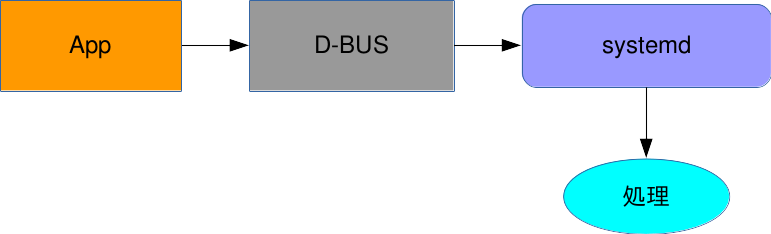
\includegraphics[width=1\hsize]{image201510/shim0.png}
\end{frame}

\begin{frame}{sysvinit$B$X$N@Z$jBX$((B}
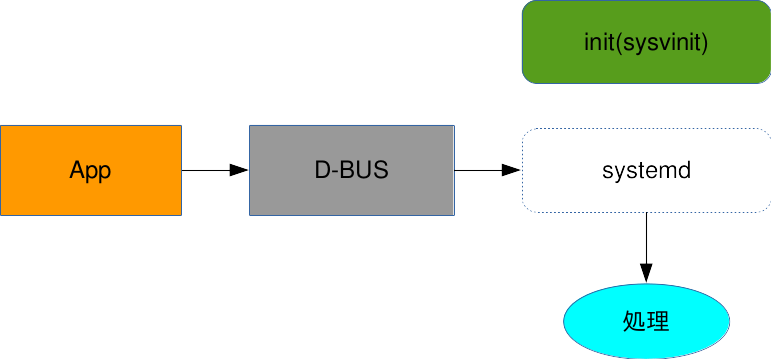
\includegraphics[width=1\hsize]{image201510/shim1.png}
\end{frame}

\begin{frame}{sysvinit$B$X$N@Z$jBX$((B}
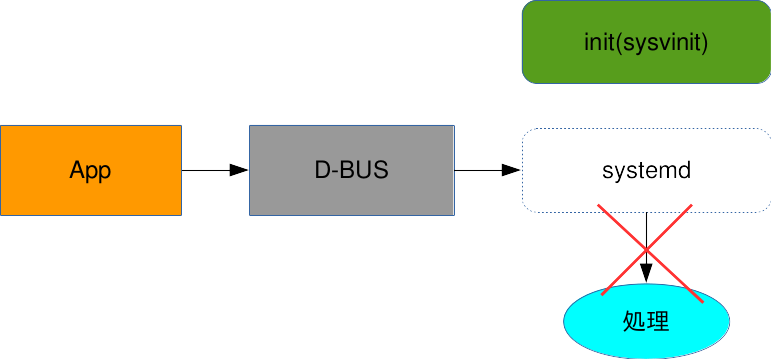
\includegraphics[width=1\hsize]{image201510/shim2.png}
\end{frame}

\begin{frame}{sysvinit$B$X$N@Z$jBX$((B}
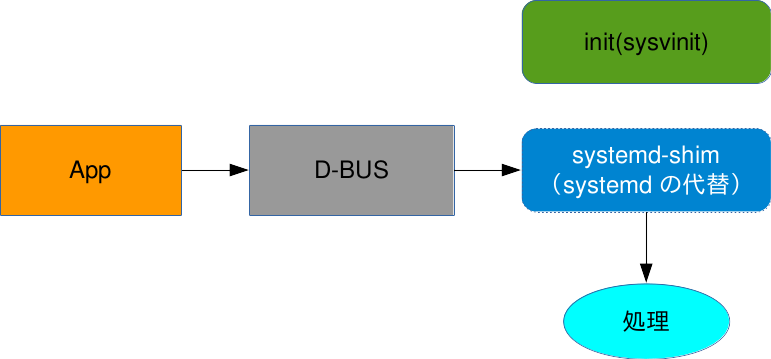
\includegraphics[width=1\hsize]{image201510/shim3.png}
\end{frame}

%\begin{frame}[containsverbatim]
%
%systemd $B$N>l9g$O(Bshutdown $B$O0J2<$N$h$&$K<B9T$5$l$k$,!"(B
%\begin{commandline}
%$ gdbus call -y -d org.freedesktop.systemd1 \
%	-o /org/freedesktop/systemd1 \
%    	-m org.freedesktop.systemd1.Manager.StartUnit \
%	'shutdown.target' ''
%\end{commandline}
%
%\item cgroup $B$O(B cgmanager $B$G4IM}!#(Bcgm $B%3%^%s%I$r;H$C$F=hM}!#(B
%\end{itemize}
%
%\end{frame}

\begin{frame}[containsverbatim]{sysvinit $B%9%/%j%W%H(B}

\begin{itemize}
\item systemd $B$K$J$C$?$i(B /etc/init.d $B0J2<$O$I$&$J$k$N$+(B
\item /lib/lsb/init-functions $B$K$h$k%i%C%Q!<$,$"$k(B
\item apache2 $B$rNc$K$7$F@bL@(B

\end{itemize}

\end{frame}


%
%\begin{commandline}
%67 if [ -f /etc/default/rcS ]; then
%68         . /etc/default/rcS
%69 fi
%70 . /lib/lsb/init-functions
%71 
%72 
%73 # Now, set defaults:
%74 APACHE2CTL="$ENV apache2ctl"
%\end{commandline}
%
%\end{frame}
%
%\begin{frame}[containsverbatim]
%
%\texttt{/lib/lsb/init-functions}
%
%\begin{commandline}
%425 log_action_end_msg_post () { :; }
%426 
%427 # Include hooks from other packages in /lib/lsb/init-functions.d
%428 for hook in $(run-parts --lsbsysinit --list /lib/lsb/init-functions.d
%2>/dev/null); do
%429     [ -r $hook ] && . $hook || true
%430 done
%431 
%432 FANCYTTY=
%\end{commandline}
%
%\end{frame}
%
%
%
%\begin{frame}[containsverbatim]
%
%\texttt{/lib/lsb/init-functions.d/40-systemd}
%
%\begin{commandline}
%_use_systemctl=0
%if [ -d /run/systemd/system ]; then
%
%    if [ -n "${DPKG_MAINTSCRIPT_PACKAGE:-}" ]; then
%    # If we are called by a maintainer script, chances are good that a
%    # new or updated sysv init script was installed.  Reload daemon to
%    # pick up any changes.
%        systemctl daemon-reload || true
%    fi
%
%    # Redirect SysV init scripts when executed by the user
%    if [ $PPID -ne 1 ] && [ -z "${init:-}" ] && [ -z
%"${_SYSTEMCTL_SKIP_REDIRECT:-}" ]; then
%        case $(readlink -f "$0") in
%            /etc/init.d/*)
%                _use_systemctl=1
% 
%
%$B!JCfN,!K(B
%
%systemctl_redirect () {
%    local s
%    local rc
%    local prog=${1##*/}
%    local command=$2
%
%    case "$command" in
%        start)
%            s="Starting $prog (via systemctl)"
%            ;;
%        stop)
%            s="Stopping $prog (via systemctl)"
%            ;;
%        reload|force-reload)
%            s="Reloading $prog configuration (via systemctl)"
%            ;;
%        restart)
%            s="Restarting $prog (via systemctl)"
%            ;;
%    esac
%
%    service="${prog%.sh}.service"
%
%$B!JCfN,!K(B
%
%    [ "$command" = status ] || log_daemon_msg "$s" "$service"
%    /bin/systemctl $sctl_args $command "$service"
%    rc=$?
%    [ "$command" = status ] || log_end_msg $rc
%
%    return $rc
%}
%
%if [ "$_use_systemctl" = "1" ]; then
%    # Some init scripts use "set -e" and "set -u", we don't want that
%    # here
%    set +e
%    set +u
%
%    if  [ "x$1" = xstart -o \
%        "x$1" = xstop -o \
%        "x$1" = xrestart -o \
%        "x$1" = xreload -o \
%        "x$1" = xforce-reload -o \
%        "x$1" = xstatus ] ; then
%
%        systemctl_redirect $0 $1
%        exit $?
%    fi
%fi
%\end{commandline}
%
%\end{frame}
%
%
%\begin{frame}[containsverbatim]
%
%\begin{commandline}
%$ sudo /etc/init.d/networking restart
%[....] Restarting networking (via systemctl): networking.serviceWarning: networking.service changed on disk. Run
%'systemctl daemon-reload' to reload units.
%. ok 
%
%\end{commandline}
%
%\end{frame}
%
%\begin{frame}
%	systemd $BBP1~%G!<%b%s(B
%	$BBP1~N((B
%
%	sysvinit $B$H(B systemd $B$NBP1~J}K!$K$D$$$F(B
%
\begin{frame}
\begin{center}
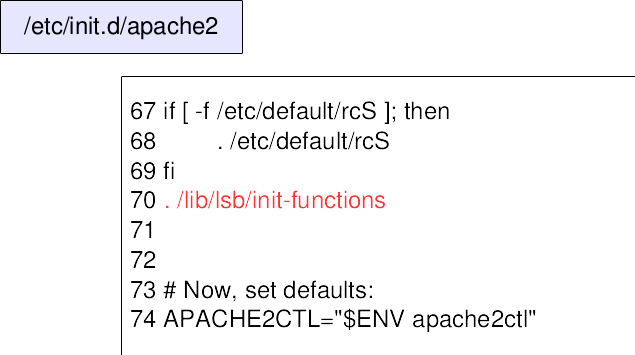
\includegraphics[width=0.8\hsize]{image201510/daemonscript0.png}
\end{center}
\end{frame}

\begin{frame}
\begin{center}
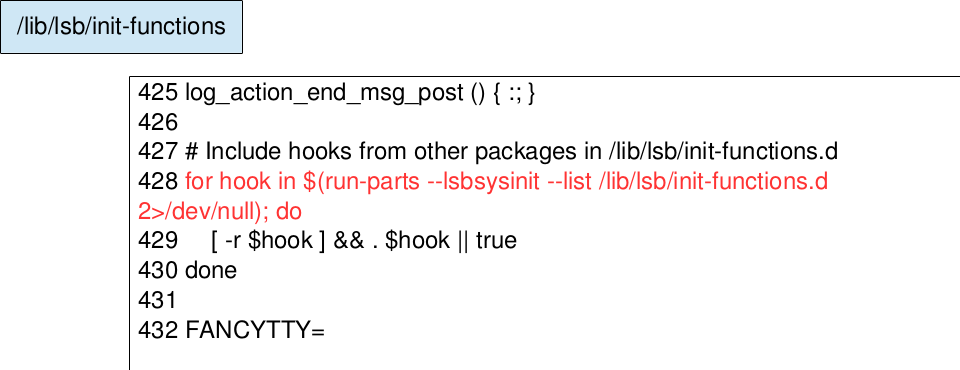
\includegraphics[width=1\hsize]{image201510/daemonscript1.png}
\end{center}
\end{frame}

\begin{frame}
\begin{center}
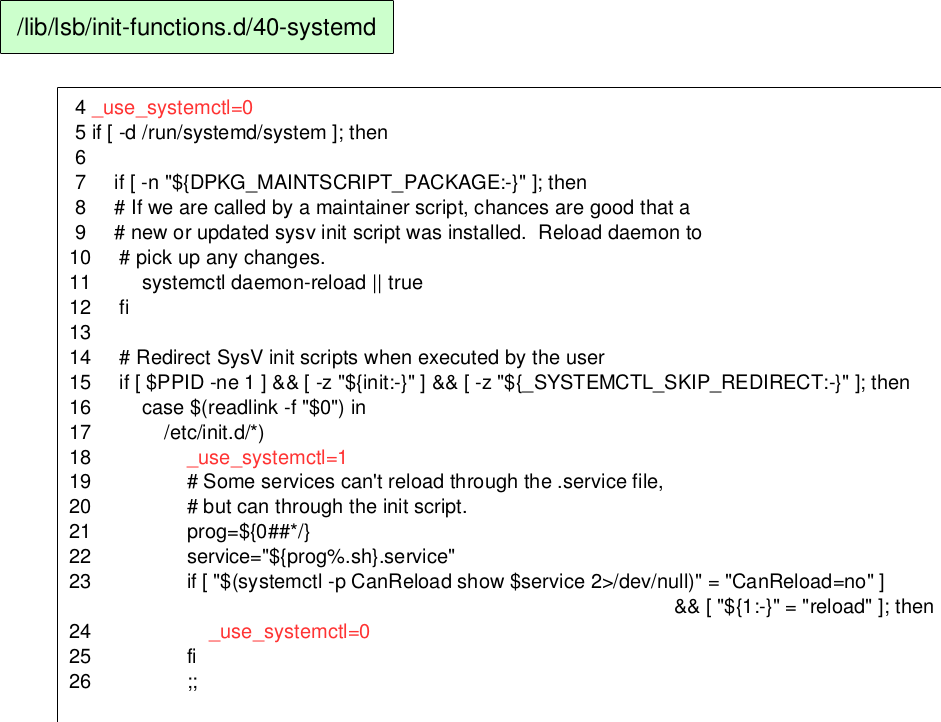
\includegraphics[width=1\hsize]{image201510/daemonscript2.png}
\end{center}
\end{frame}

\begin{frame}
\begin{center}
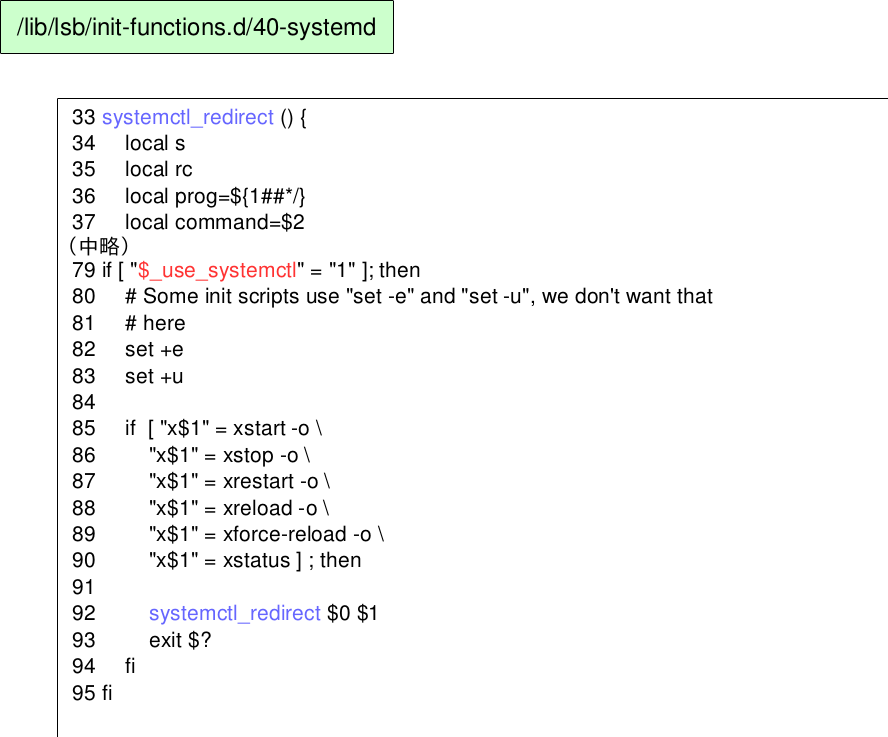
\includegraphics[width=1\hsize]{image201510/daemonscript3.png}
\end{center}
\end{frame}

\begin{frame}
\begin{center}
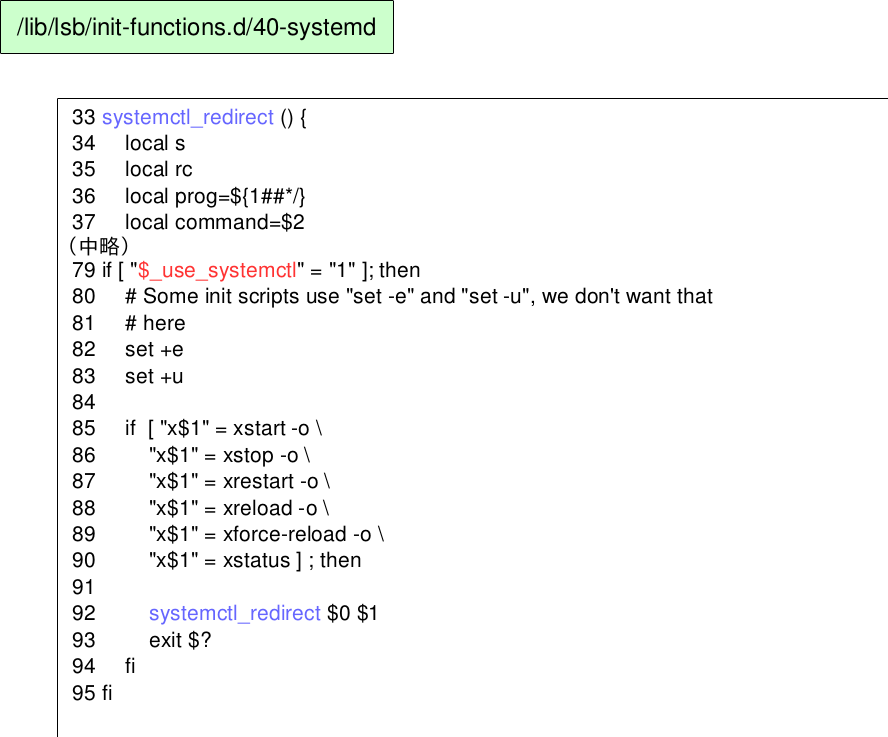
\includegraphics[width=1\hsize]{image201510/daemonscript3.png}
\end{center}
\end{frame}

\begin{frame}
\begin{itemize}
\item /lib/lsb/init-functions $B$r;H$C$F$J$$%G!<%b%s$,$"$k$N$G$O!)(B
\item lintian $B$N(B \texttt{init.d-script-does-not-source-init-functions} $B$K0z$C$+$+$C$F$$$k$b$N$OMWCm0U(B

\url{https://lintian.debian.org/tags/init.d-script-does-not-source-init-functions.html}
\end{itemize}
\end{frame}

\begin{frame}{$B$^$H$a(B}

\begin{itemize}
\item Debian $B$G$O(B systemd $B$r;H$o$J$$$G1?MQ$G$-$k(B
\item systemd $B$r:o=|$7$?>l9g$O(Bsystemd-shim $B$r%$%s%9%H!<%k$7$F$*$/$H$h$$(B
\item $B%5!<%S%94XO"$O$$$^$^$G$N%3%^%s%I$,$=$N$^$^;H$($k(B
\item /etc/init.d/ $B0J2<$O(B systemd $B$H(B sysvinit $B$G$bN>J};H$($k$h$&$K$J$C$F$$$k(B
\end{itemize}

\end{frame}

\section{$B<ALd(B}
\emtext{$B<ALd(B}
\begin{frame}{$B<ALd(B}
$B2?$+<ALd$O$"$j$^$9$+!)(B
\end{frame}

\section{$B%V!<%9(B}
\emtext{$B%V!<%9(B}
\begin{frame}{$B%V!<%9=P$7$F$$$^$9(B}
$B%V!<%9=P$7$F$$$^$9!#$h$+$C$?$i4s$C$F$/$@$5$$!*(B
\end{frame}

\section{$B:#8e$N%$%Y%s%H(B}
\emtext{$B:#8e$N%$%Y%s%H(B}
\begin{frame}{$B:#8e$N%$%Y%s%H(B}
\begin{itemize}
\item 2015/11/7 ($BEZ(B) KOF 2015 $B=PE8(B\&$BH/I=!#(B\\
\url{https://k-of.jp/2015/}
\item 2015/11/21($BEZ(B) 14:00-19:00 $BBh(B133$B2sEl5~%(%j%"(BDebian$BJY6/2q(B
\end{itemize}
\end{frame}


\end{document}

;;; Local Variables: ***
;;; outline-regexp: "\\([ 	]*\\\\\\(documentstyle\\|documentclass\\|emtext\\|section\\|begin{frame}\\)\\*?[ 	]*[[{]\\|[]+\\)" ***
;;; End: ***
